%======================================================================
\section{Physical Unclonable Functions - \pufs~}
\label{sec:pufs}
It is well known that every time an Integrated circuit(IC) is fabricated there are small random process variations, imperfections that make every path in a design unique, for a design where the goal is to have always the same behavior for all ICs, these imperfections are measured and errors are avoided by creating timing constraints that will guide the Electronic Design and Automation(EDA) tools to  generate error-free paths and deliver a \rm{secure} robust design. \pufs~are physical functions that instead of avoiding, take advantage of this inherent imperfections to mimic random functions. Their inputs, called challenges, and outputs, called responses, are designed to have a unique relationship for every \puf~instance.\mario{Add a reference to puf in general }

\subsection{\puf~ Types}
\mario{Add a  puf summary with puf types and say that you are going to describe two }
It is possible to explore IC process variations in several ways\cite{DBLP:phdbasesearchMaes12}, a great and simple example to understand the behavior of these functions is an arbiter PUF, pictured in Figure \ref{fig:arbiterpuf}.
This \puf~ is composed by a set of crossbar switches and one arbiter, the flip-flop\mario{Change the figure to a flip flop and add devadas reference}. The idea behind this construction is to build two paths with the same layout length and compute the relative delay between these two paths given a challenge $X$ of size $N$.  For every switch $n$, if $X[i]$  is one both paths will pass through the arbiter, if its zero the inputs will be switched in the output changing the delay of booth paths. To evaluate the output(Y), the challenge $X$ and a rising signal are provided to both paths, $Y$ is one if the signal to the latch data input (D) is faster, and zero otherwise. To get a response of size $Z$, this \puf~ construction  can be instantiated $Z$ times.

\begin{figure*}[!ht]
	\centering
% 	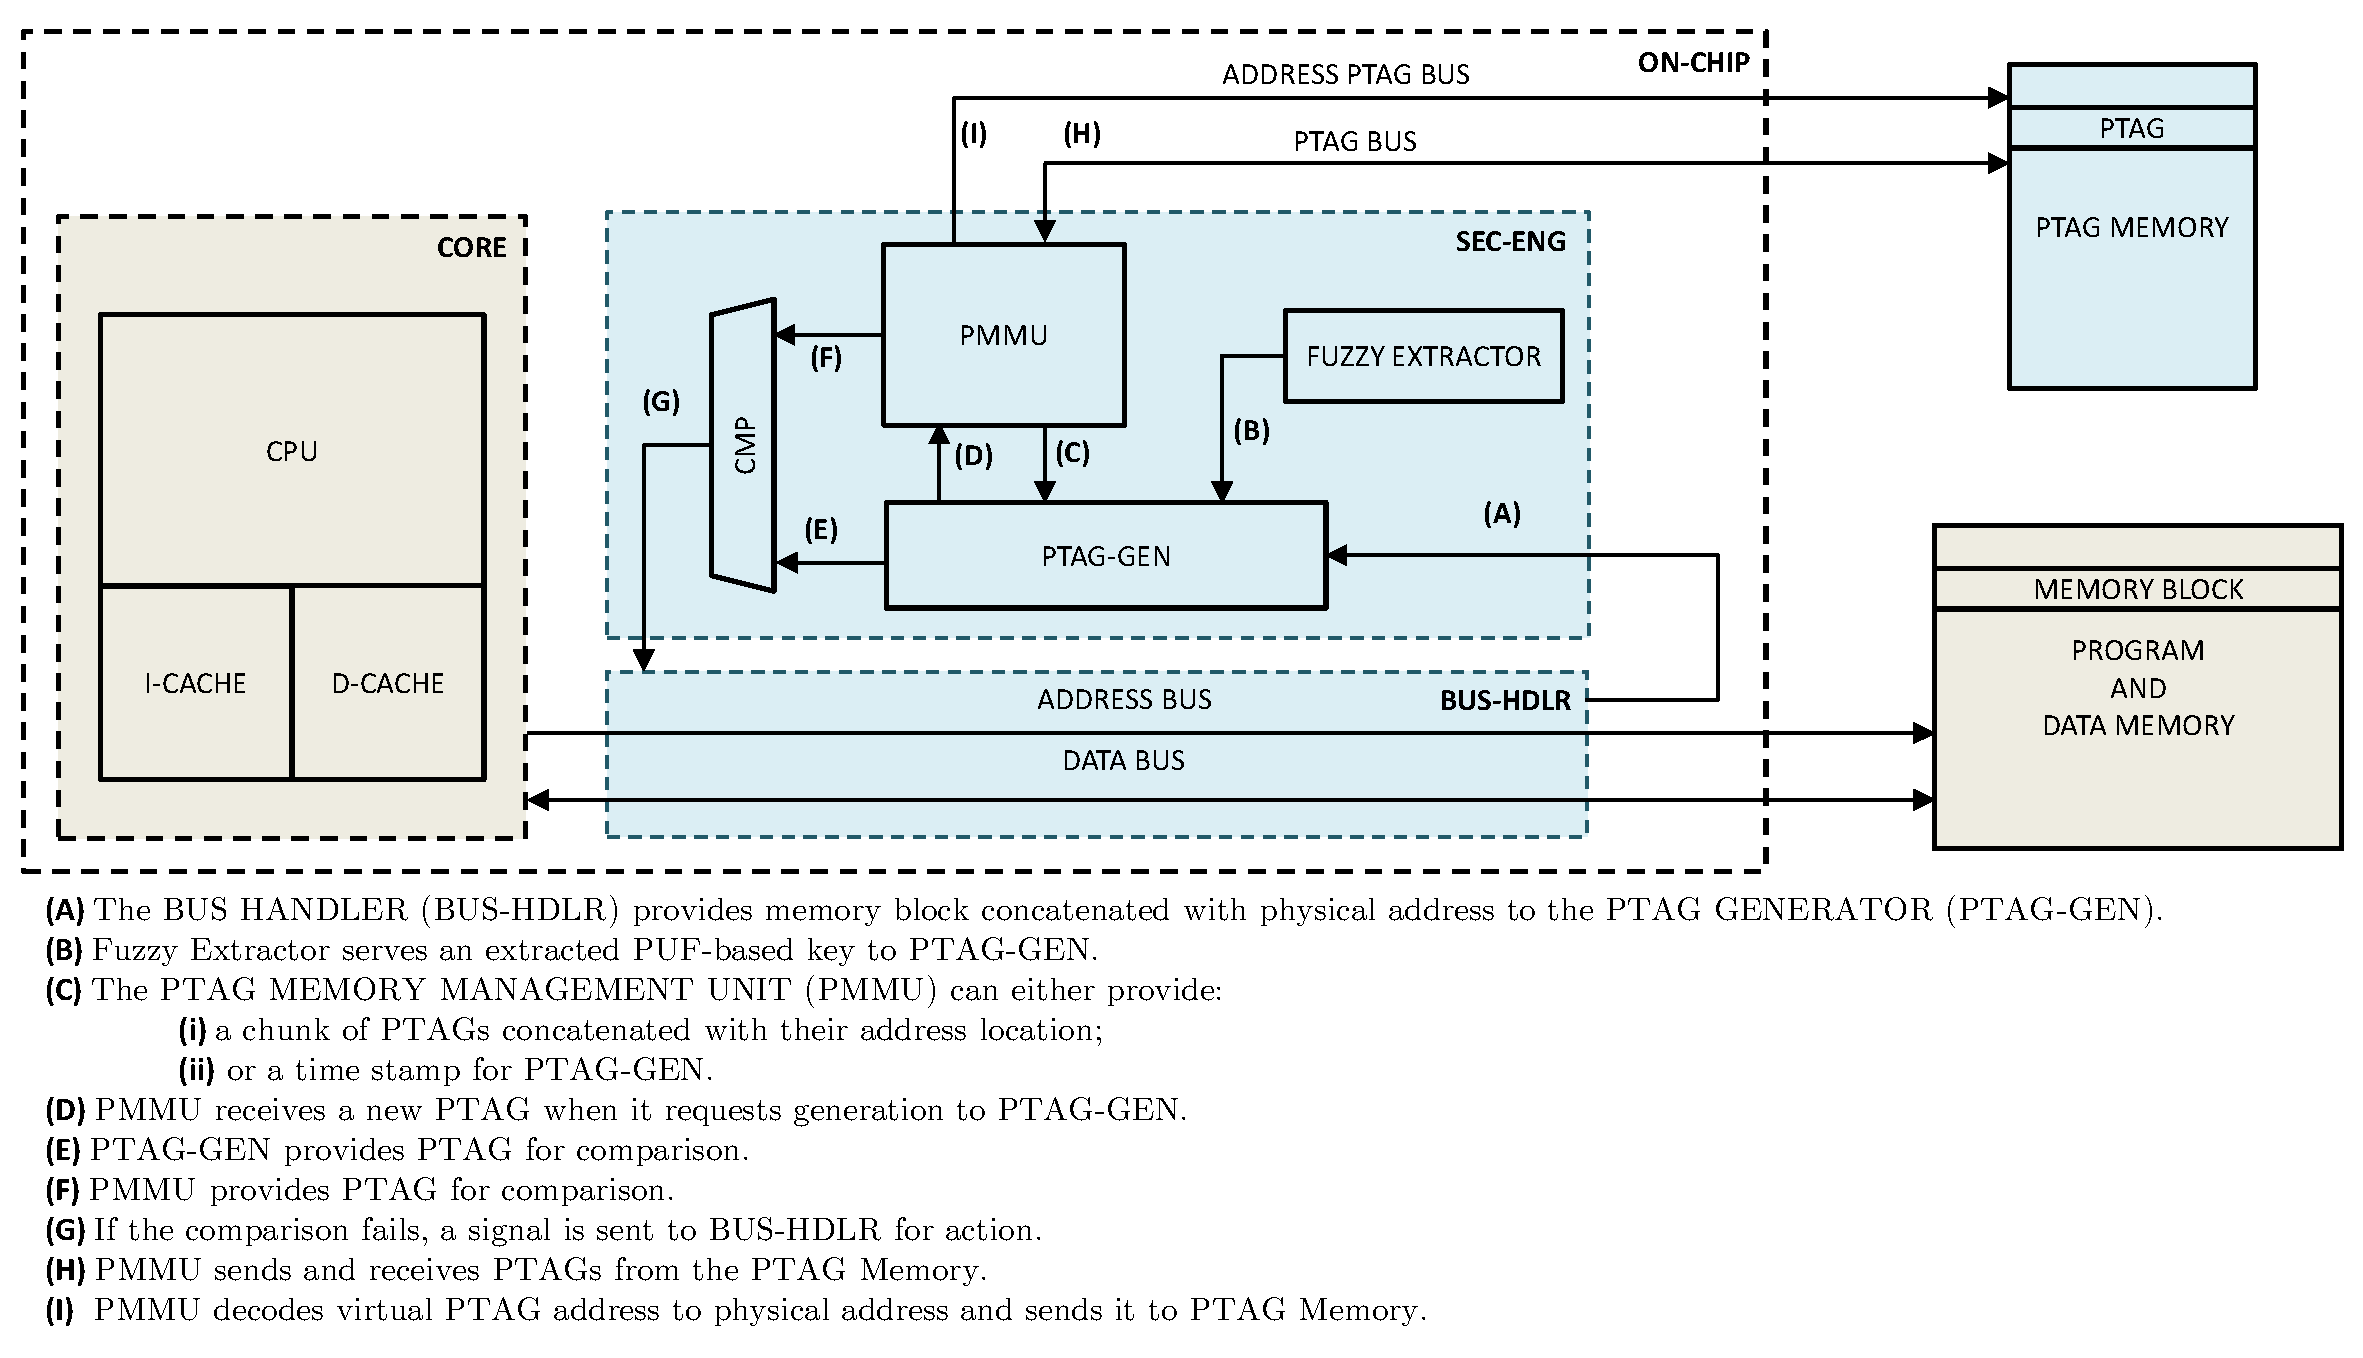
\includegraphics[scale=0.45]{cshia}
	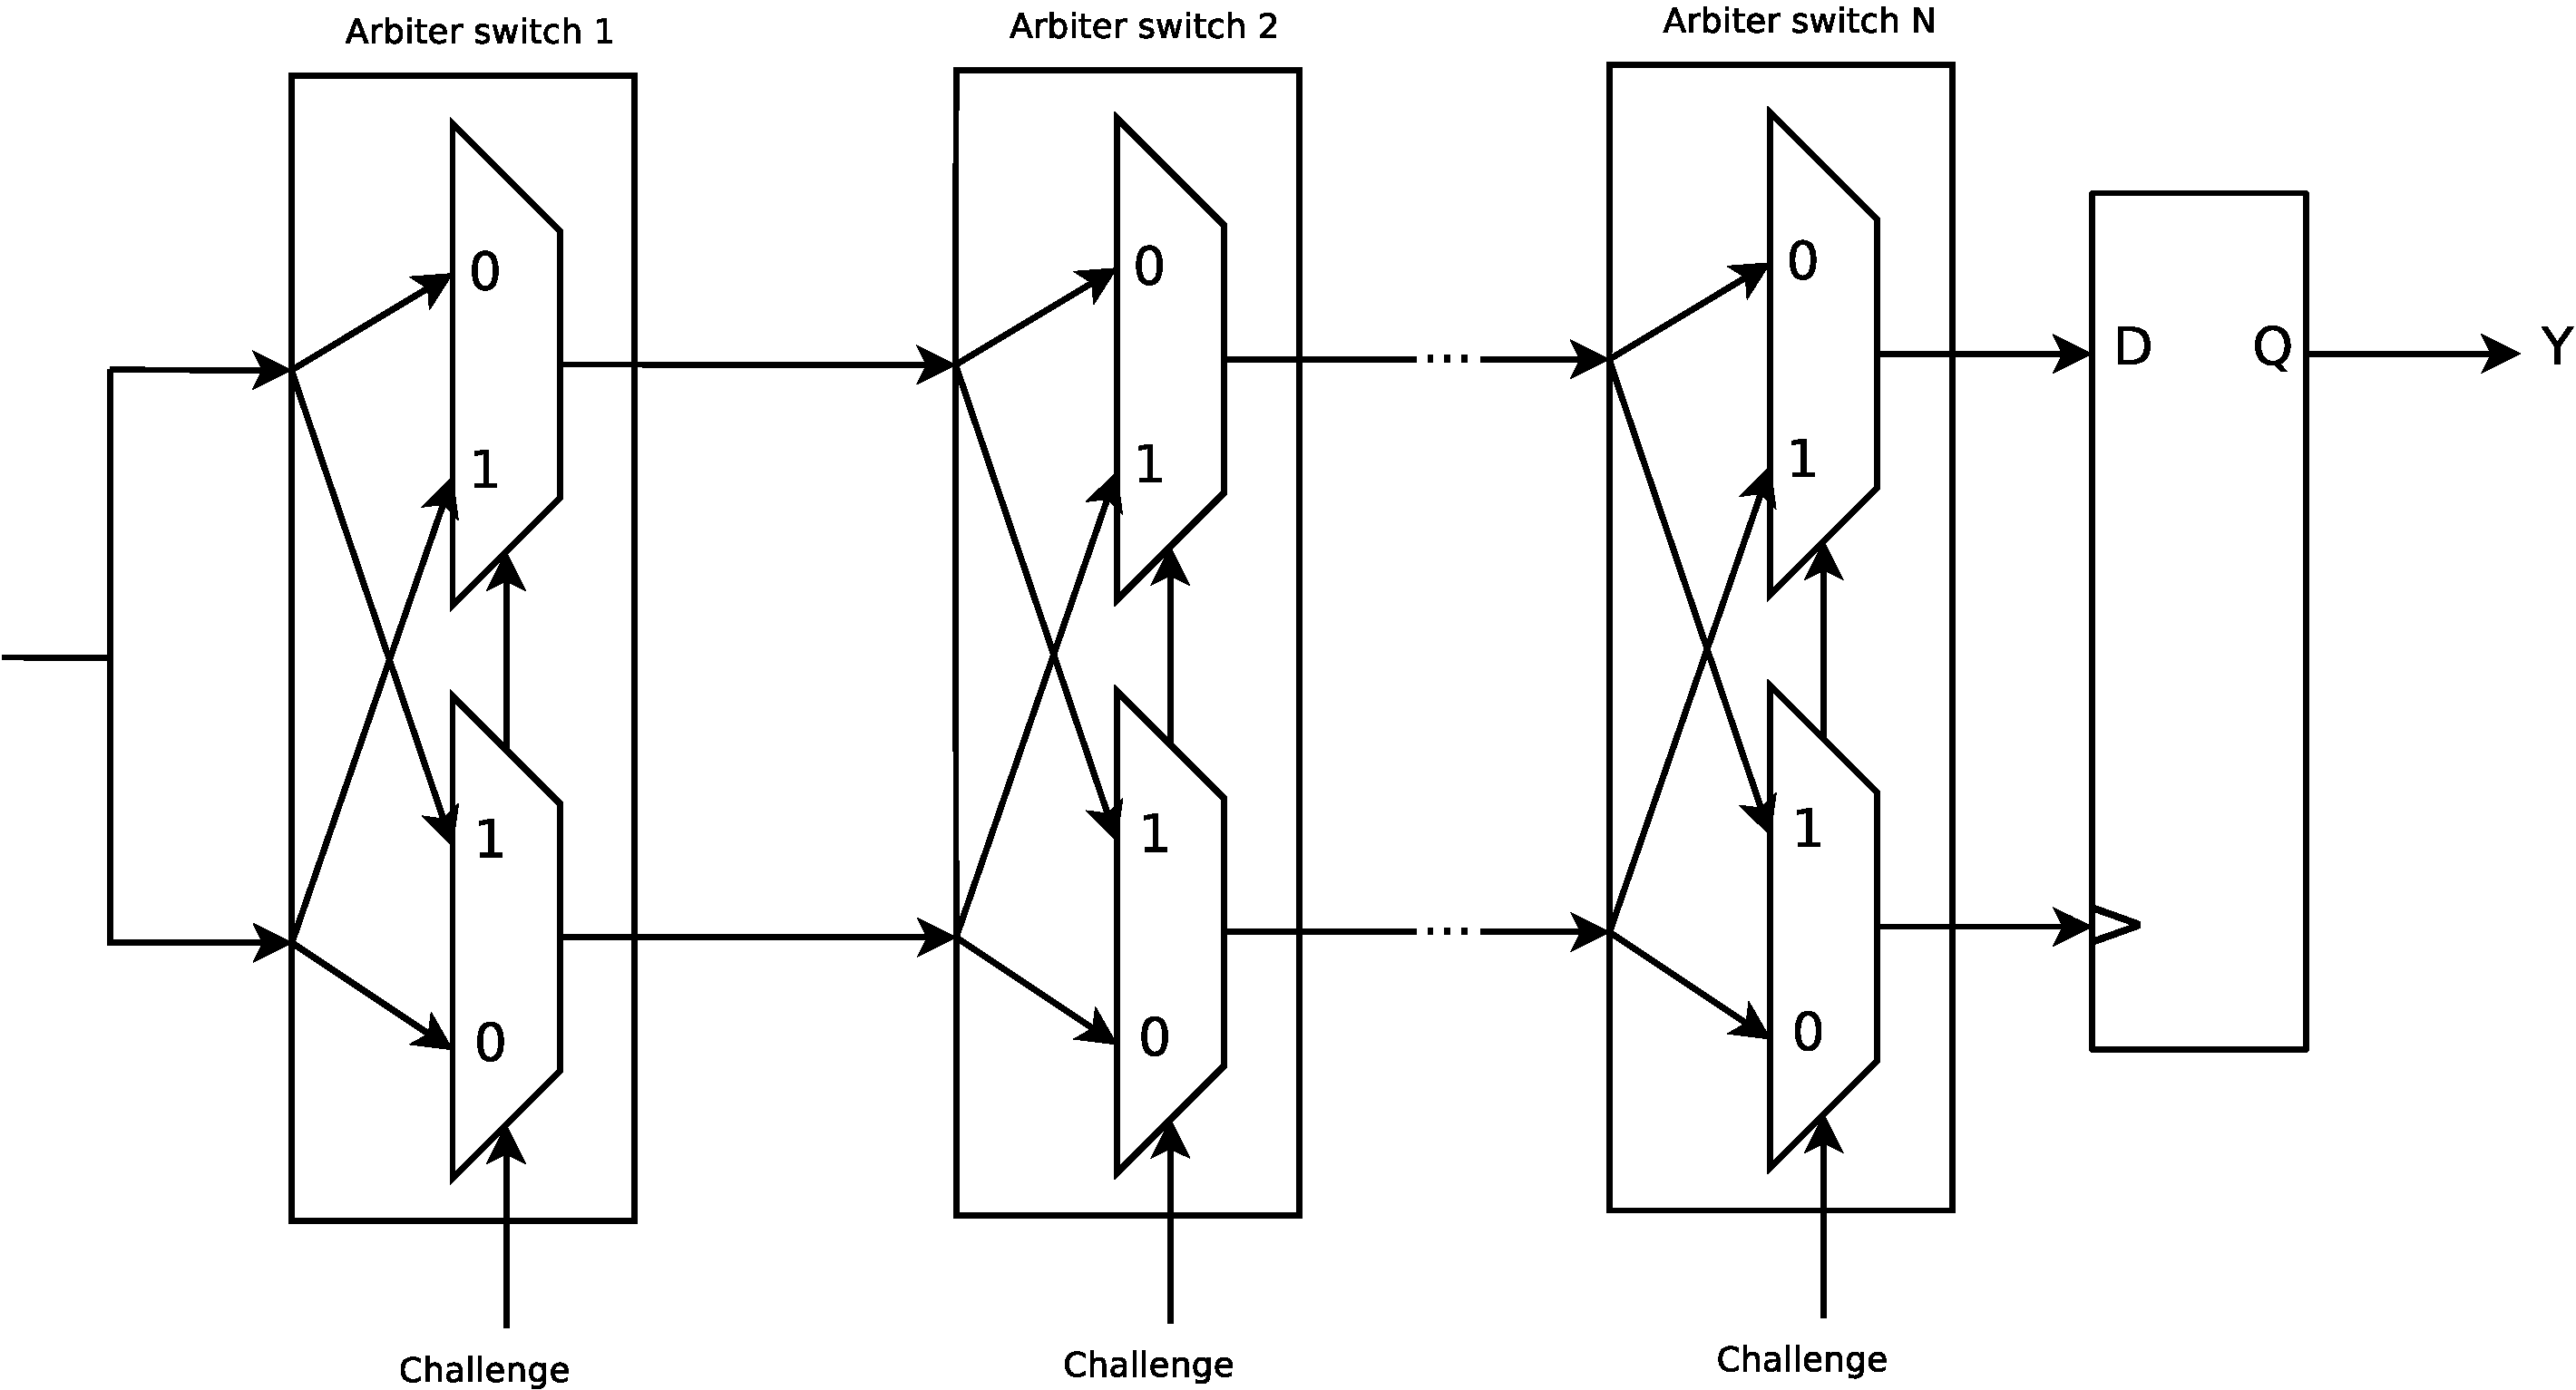
\includegraphics[width=0.85\textwidth]{arbiter}
	\caption{One arbiter \puf~ that receives a challenge $X$ and produces the output $Y$.}
%	\vspace*{-9pt} 
	\label{fig:arbiterpuf}
\end{figure*}

Another \puf~ type is the Static Random-Access Memory (SRAM) \puf~ \mario{Cite the author properly}\cite{Leest2012}, in this model, each SRAM cell within an SRAM block can be considered a \puf~. The typical cell implementation, shown in Figure \ref{fig:spufexample} is built from two cross-coupled inverters at its core, from an electronic viewpoint, this circuit contains a positive feedback loop which reinforces its current state. In a logic sense, this circuit has two stable values (bistable), and by residing in one of both states the cell stores one binary digit.\mario{reduce the technical part and explain the concepts in a higher level}

The operation principle of an SRAM PUF is based on the transient behavior of an SRAM cell when it is powered up, i.e., when its supply voltage Vdd comes up. The circuit will evolve to one of its operating points, but it is not immediately clear to which one. In Figure   \ref{fig:spufexample} the inverters $I_1$ and $I_2$ have its drive strength determined by the process variations when this memory was manufactured, these inverters will compete to achieve stability. When one of the inverters is significantly stronger than the other one, the preferred initial operating point will be a stable state, and the preference will be very distinct, i.e., such a cell will always power-up in the same stable state, but which state this is (‘0’ or ‘1’), is randomly determined for every cell.
So in a \puf~ that uses an SRAM, the challenge is the row and column addresses, the output is the state of the cell after power up.
\begin{figure*}[!ht]
	\centering
	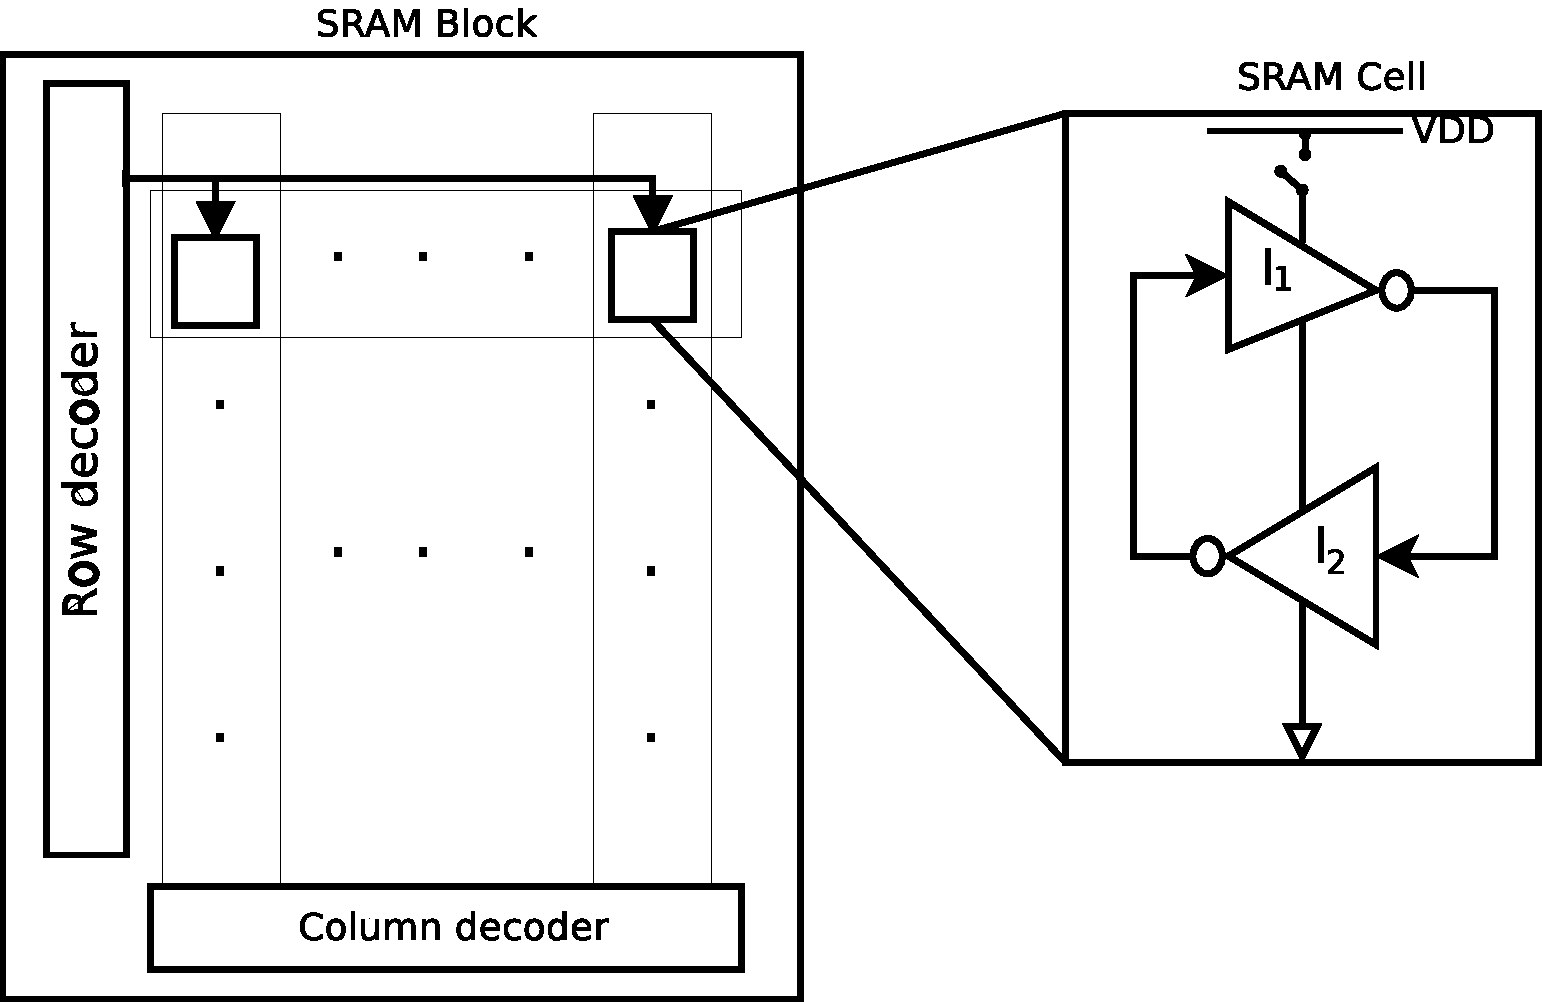
\includegraphics[scale=0.42]{figures/pdf/spuf}
% 	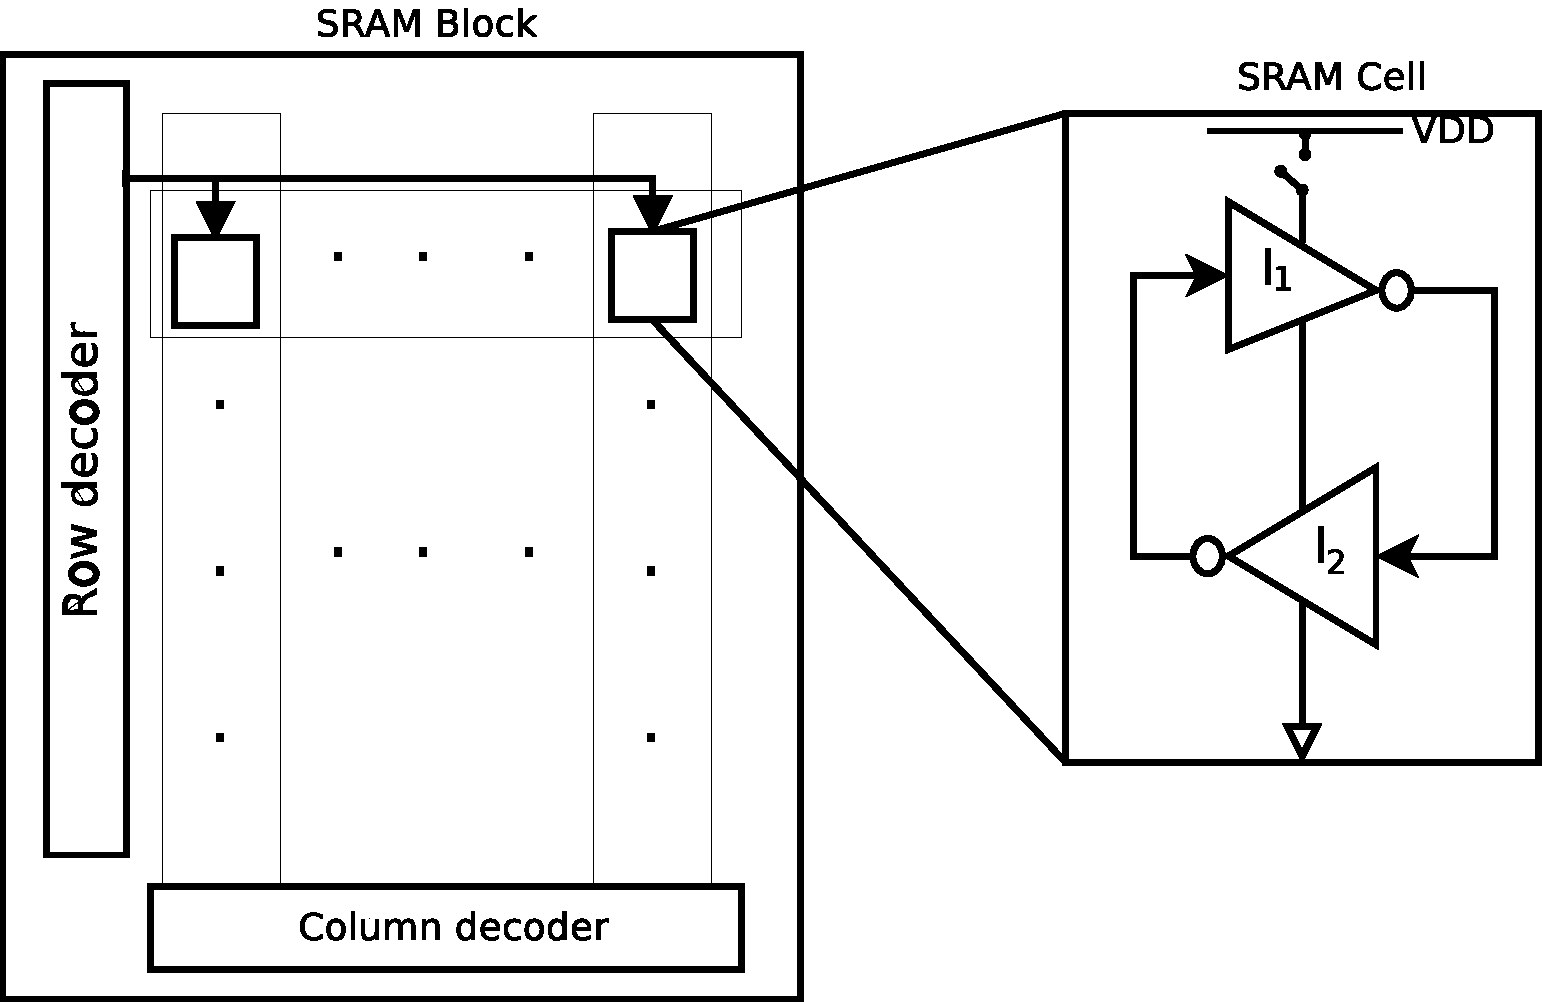
\includegraphics[width=\textwidth]{figures/pdf/spuf}
	\caption{A simplistic example of a SRAM \puf~ , showing the SRAM cell logic circuit inside an SRAM block.}
%	\vspace*{-9pt} 
	\label{fig:spufexample}
\end{figure*}


\subsection{\puf~ as a Cryptographic  Key Generator }
When a system needs a key in hardware for any purpose, such as encryption, authentication, or any other application, this key needs to be generated and stored in hardware \cite{puf-key-devadas-1278484}. The main advantage of using \pufs~as key generators is that they can produce keys at running time, this way, on-chip memories are not needed for key storage. Another benefit is that they are unclonable, meaning that even the manufacturer itself cannot produce two \puf~instances that will have the same set of Challenge-Response Pairs (\crps) \cite{Gassend2002:PUFs}. \mario {Better not to mix the work with the concepts}
\rem{\cshia~ uses a SRAM \puf~ together with a Fuzzy Extractor and the key extraction process is described in Section \ref{subsubsec:Key-Extraction}.}


%======================================================================
\section{Security Properties}
\label{sec:securityproperties}
In order to build a robust system, a designer has at his disposal mechanisms that implements three security properties: \mario{Briefly  introduce the concepts here and check the correct definition of each for instance : Preservation of confidentiality , integrity and availability of information, in addition other properties, such as authenticity, accountability, non-repudiation and reliability can also be involved (ISO/IEC 27000:2009)}authenticity, integrity, and secrecy. Although these features can be implemented through software, the stringent nature of embedded systems demands solutions that consume few clock cycles and are not power consuming.
In the following, we discuss hardware implementation of those security features.

%---------------------------------------------------------
\subsection{Authenticity}
\label{subsec:Authenticity}
Suppose that an attacker wants to add \hisher~own code for execution in the embedded system or intends to move the data from one system instance to another. These attacks can be avoided by employing authentication mechanisms. In this solution, a key (or unique set of keys) is determined for each instance.
%TODO explain the instance more clear
Code \andor~ data are tagged using these keys during manufacturing \rem{(an enrollment phase)}. \mario{this is typical of integrity } \ed{At run time, this key (or set of keys) is used to regenerate tags. Only a correct key value will be able to verify what was installed during manufacture. Therefore, an instance will not accept code or data that was not tagged using its own keys.}

Before the introduction of electronic \pufs \cite{Gassend2002:PUFs}, these keys had to be inserted into the system before they were made available to the users. To do so, keys are stored on-chip using non-volatile memories and the manufacturer\slash{}vendor controlled the uniqueness of the keys in each instance. The main downsides of storing key permanently include: facilitating physical attacks \cite{Sadeghi2010:Security-PUFs}, and possibly increasing costs of production since it may demand integration of different technologies on the same chip.

%---------------------------------------------------------
\subsection{Integrity}
\label{subsec:integrity}
\ref{subsec:integrity}
Similarly to authentication, integrity is ensured by tagging code and data with additional information such as memory address location \andor~timestamps. This prevents an attacker from tampering with a system by, for instance, moving instructions from their location in memory, setting different initial values of variables, etc. The level of integrity can be done for an entire program, memory pages, or memory blocks. 

Integrity can also be considered at the instruction sequence level, which we refer as Control-Flow Integrity (CFI). Hardware solutions for control-flow integrity usually require deep integration between hardware and software \cite{Davi2015:HAFIX}, that can result not only in changing the Instruction Set Architecture (\isa) \andor~the tool-chain, but also the processor's data path, as proposed in \cite{Gelbart2005:CODESSEAL, Kanuparthi2012:DynamicIntegrity}. Even though CFI protection is welcomed, many embedded system applications cannot afford the performance penalties and storage overhead inherently of this solution. For instance, in applications where user inputs are limited and \io~involves fixed amounts of data, an attacker has very little room to employ a buffer overflow or similar attacks prevented by CFI. However, integrity verification regarding blocks of code and data (as mentioned above) can avoid a variety of situations that go beyond run time attacks. For example, if an embedded system is unwatched, an attacker can upload malicious code or modify the data in the external memory even if the system is not running. Integrity verification can prevent and indicate these violations before they reach the processor.


%---------------------------------------------------------
\subsection{Secrecy}
\label{subsec:Secrecy}

An embedded system can also use encryption to prevent exposure of code \andor~data stored in the external memory. Consequently, the processor can run these instructions and data only after decryption. Therefore, the major drawback of using encryption is the performance overhead that highly depends on which cryptographic primitive is employed \cite{Suh2007:PUFs}. Also, secrecy only prevents that an attacker obtains the information, if it is not combined with a unique key or integrity verification, the system will be vulnerable to execute code of different system instances \andor~to suffer \mario{Explain attacks?} \ed{relocation and replay attacks\cite{Elbaz2009}.}

\mario{It is common to end each chapter with a closure,  in a higher abstraction level do a connections with  the next chapters }